\chapter{Takel mechanisme}

\section{Contragewicht}
Een contragewicht(zie figuur~\ref{fig:contragewicht}) is een gewicht dat even zwaar is als de lift bij een gemiddelde lading. Als het gewicht van de lift wordt genomen en het gemiddelde gewicht van de lading, is dat het beste gewicht voor een contragewicht. Door een contragewicht te gebruiken hoeft de motor niet veel arbeid te leveren. Het gewicht van de lift is door het contragewicht opgeheven. 

\section{Spoel}\label{sec:spoel}
Een spoel(zie figuur~\ref{fig:spoel}) werkt door de lift aan een rol vast te binden en het touw omhoog te trekken samen met de lift om de lift te verplaatsen. het voordeel hiervan is dat dit een simpel systeem is. Deze methode kan al worden geïmplementeerd met alleen een motor, spoel en de lift aan een touw. Ook is de geleiding van alleen een lift makkelijker dan een lift met contragewicht. Je hoeft immers alleen rekening te houden met de lift zelf in plaats van de lift die zijn eigen plek heeft en het contragewicht.
\\
\begin{figure}[ht]
\begin{subfigure}{0.5\textwidth}
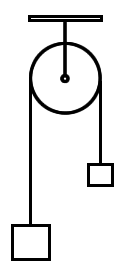
\includegraphics[height=5cm]{src/contragewicht} 
\caption{Contragewicht}
\label{fig:contragewicht}
\end{subfigure}
\hfill
\begin{subfigure}{0.5\textwidth}
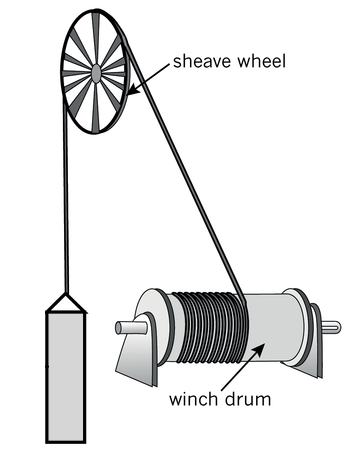
\includegraphics[height=5cm]{src/spoel}
\caption{Spoel}
\label{fig:spoel}
\end{subfigure}
\caption{Schematische weergave van takel mechanisme}
\label{fig:takel_mechanisme}
\end{figure}

\section{Voor- en nadelen}
\begin{center}
\begin{tabular}{l|c|c}
& Contragewicht & Spoel \\
\hline
Krachtige motor nodig & \xmark & \cmark \\
\hline
Complexe liftconstructie & \cmark & \xmark \\
\hline
Prijs & \euro{5} - \euro{10} & \euro{3} - \euro{6}
\end{tabular}
\end{center}

\section{Advies}
Hierbij adviseren wij een spoel. Dit omdat de spoel naar ons mening minder bouw \& ontwerp problemen met zich mee brengt dan een contragewicht.